\documentclass{article}
\usepackage{xcolor}
\definecolor{darkgreen}{rgb}{0.0, 0.5, 0.0}
\usepackage[utf8]{inputenc}
\usepackage{graphicx}
\usepackage{subcaption} % Use subcaption instead of subfigure
\usepackage{matlab-prettifier}
\usepackage{amsmath}



% Set equation numbering to section and subsection
%\renewcommand{\theequation}{\thesubsection.\arabic{equation}}
\makeatletter
\@addtoreset{equation}{subsection}
\makeatother
\usepackage{listings}
\usepackage{amssymb}
\usepackage{blindtext}
\usepackage{geometry}
\usepackage{graphicx}
\usepackage{float}
\usepackage{dirtytalk}
\usepackage{enumitem}
\usepackage{derivative}
\usepackage{biblatex}

\usepackage{svg}  % Enables SVG support
\usepackage{hyperref} % Enables hyperlinks
% No red boxes at hyperlinks
\hypersetup{
    colorlinks,
    linkcolor={blue},
    citecolor={blue},
    urlcolor={blue}
}

\lstset{
    language=Python,             % The language of the code
    basicstyle=\ttfamily\small,  % The font style for the code
    keywordstyle=\color{blue},   % Color of Python keywords
    stringstyle=\color{darkgreen},     % Color of strings
    commentstyle=\color{gray},  % Color of comments
    showstringspaces=false,      % Do not show spaces in strings
    frame=single,                % Frame around the code
    numbers=left,                % Line numbers on the left
    numberstyle=\tiny\color{gray},  % Style of the line numbers
    breaklines=true,             % Automatic line breaking
}%Imports biblatex package
 \geometry{
 a4paper,
 total={160mm,250mm},
 left=25mm,
 top=30mm,
 footskip =10mm,
 }

\title{Monte Carlo Simulation - Portfolio loss and importance sampling}
\author{Thomas Sejer Canham}

\date{\today} 
\setlength\parindent{0pt}

 \begin{document}

\begin{titlepage}
 \maketitle
 \centering{Aarhus University}
 %Table of contents
 \tableofcontents
 \thispagestyle{empty}
\end{titlepage}
\section{Introduction}

In this project, we will investigate the use of Monte Carlo simulation (MCS)  to estimate the exceedance probability $\mathbb{P}(L > x)$ of a loss $$ L = \delta^T\Delta S + \Delta S^T\Gamma\Delta S,$$
where, $delta \in \mathbb{R}^m$, $\Gamma \in \mathbb{R}^{m\times m}$ and $\Delta S \sim \mathcal{N}(0, \Sigma_S)$ is a (multivariate) normal random variable. The exceedance probability is the probability that the loss $L$ exceeds a certain threshold $x = 10$. \vspace{.5cm}


In the parts $(a)$, $(b)$ and $(c)$, we will focus on the one-dimensional case, $m= 1$. These three parts will compare crude MCS with MCS where we introduce control variates and importance samplingm respectively. In part $(d)$, the differences of these methods are visuallized by comparison of the confidence intervals of the estimates that are obtained from each method. \vspace{.5cm}

Parameters for the various codes snippets can be seen in the appendix in \autoref{code_params}.

\section{Crude Monte Carlo Simulation}
In this section, we will implement a crude Monte Carlo simulation to estimate the exceedance probability $\mathbb{P}(L > x)$ for the one-dimensional case ($m=1$). We are interested in ${P}(L > x)$. We may introduce the indicator function $\mathbb{I}(L > x)$ of the event $L > x$. If we compute the expectation of the indicator function, we obtain the exceedance probability

\begin{equation}
    \mathbb{P}(L > x) = \mathbb{E}[\mathbb{I}(L > x)] = 0\cdot\mathbb{P}(L > x) + 1\cdot\mathbb{P}(L > x) = \mathbb{P}(L > x),
\end{equation}
by the bernoulli property of the indicator function. We estimate the exceedance probability by use of the following Monte Carlo estimator
\begin{equation}
    \hat\ell = \frac{1}{N}\sum_{i=1}^{N} \mathbb{I}(L_i > x) \xrightarrow[N \to \infty]{a.s} \mathbb{E}[\mathbb{I}(L > x)],
\end{equation}
by the law of large numbers. The crude Monte Carlo simulation is implemented in the code snippet seen in \autoref{code_a}. A estimate of
\begin{equation*}
    \hat{\ell} \approx 0.0103
\end{equation*}
is found with a variance of $s^2 = 1.03\cdot 10^{-7}$.


% Import the code from a.py
\lstinputlisting[
    caption={Python code for crude MCS},
    label={code_a}
]{a.py}


\section{Control Variable}
A control variable is now introduced with the aim of reducing the variance of the Monte Carlo estimator. One caviat of the control variable method is that we need a closed from expression for the expectation of the control variable. We introduce the control variable $Y = \Delta S$ and compute its expectation

\section{Comparison of the methods}

\begin{figure}[h]
    \centering
    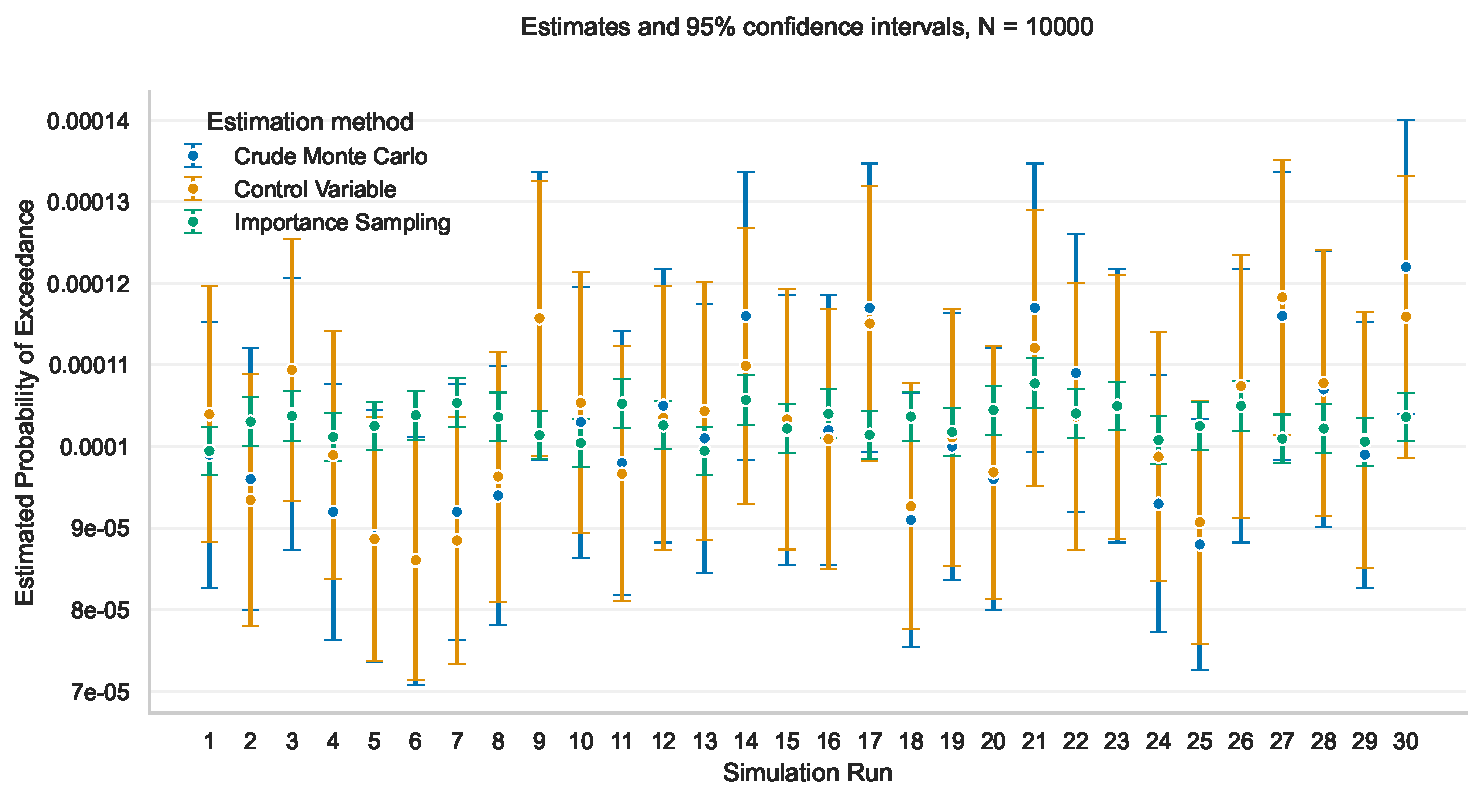
\includegraphics[width=0.9\textwidth]{figures/ConfInts.pdf}
    \caption{Comparison of confidence intervals for crude MCS, control variable MCS and importance sampling MCS. The confidence intervals are based on 30 simulations with $N = 10^4$ samples each.}
    \label{fig:my_plot}
\end{figure}







\newpage
\section{Appendix}
\lstinputlisting[
    caption={parameters.py - Parameters for the various code snippets},
    label={code_params}
]{parameters.py}



\end{document}